\chapter{Entorno de desarrollo}

Este capítulo describe el proceso seguido para establecer el entorno de desarrollo, incluyendo los problemas que se encontraron, las soluciones que se tomaron y finalmente el resultado obtenido. Este entorno servirá de base para el trabajo posterior en los siguientes capítulos que, como está descrito en la sección de condiciones de diseño, tiene como función principal habilitar la validación del trabajo realizado por medio de la técnica ``Processor-in-Loop''.

\section{Selección de autopiloto base}

Existe un requisito que inmediatamente acota la selección de autopiloto, el software debe ser de código abierto debido a que posiblemente el código se deba modificar en caso de que las opciones de configuración del autopiloto no sean suficientes para cumplir los objetivos. En el laboratorio de técnicas aeroespaciales se cuenta con hardware Pixhawk programado con el firmware de fábrica PX4.

\begin{figure}[h]
    \centering
    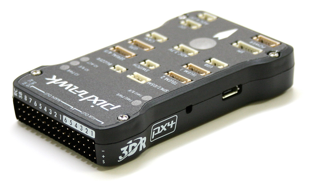
\includegraphics{hardware-pixhawk.png}
    \caption{Autopiloto Pixhawk}
    \label{fig:pixhawk1}
\end{figure}

El hardware autopiloto Pixhawk se puede programar con varias soluciones

y será provechoso si ya existen esfuerzos por agregar la capacidad de algoritmos personalizados a alguno de estos lo que reduciría trabajo. Una solución que se acerca a esta visión es la de recompilar ArduPilot junto con código exportado de Simulink para la implementación de nuevos controladores \cite{ardupilot-custom}.

\section{Extensión de protocolo de comunicación}
